\documentclass{article}
\usepackage[utf8]{inputenc}
\usepackage{graphicx}
\usepackage{amsmath}
\usepackage[]{mathabx}

\usepackage{titlesec}

\title{KombSøg Eksamensnoter 2017}
\author{Anders H Pedersen }
\begin{document}

\maketitle
\tableofcontents

\newpage

\section{P, NP and NPC.}

\subsection{Beslutningsproblemer og stand-in sprog}
I dette kursus har vi fokuseret på beslutningsproblemer, dvs. problemer hvor outputtet er yes/no.\\ Og vi har indført såkaldte stand-in sprog for de oprindelige sprog. Eksempelvis max cut, som er et optimerings problem hvor vi leder efte wr det største cut. I stand-in problemet får vi udover grafen også givet et target k, og vi spørger om der findes et cut af størrelse mindst k. Ideen er så at vi kan vise at stand-in sproget ikke har en effektiv algoritme, og dermed har det originale problem heller ikke stand-in sproget ikke er sværere end det originale(Hvis nogen påstår at det er nemmere så kan vi bruge algoritmen for det og sammenligne med vores target k, og dermed få et rigtigt svar).

\subsection{P, NP, NPC}
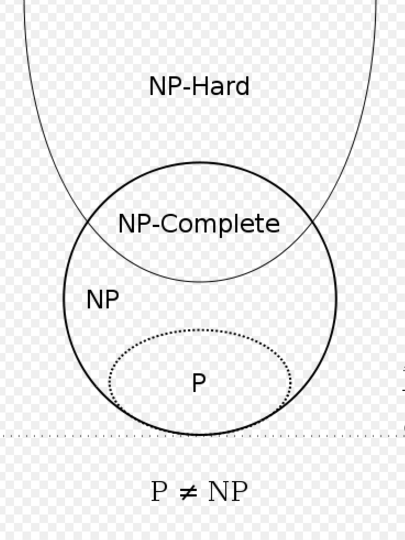
\includegraphics[scale=0.5]{asd.PNG}\\
\textbf{P} er klassen af problemer som kan løses i poly-tid af en TM. Og når vi skal argumentere for at et problem er i P, så beskriver vi en effektiv algoritme og refererer til \textbf{Polynomial Church-Turing thesis} som siger noget om at noget kan løses af en TM i poly-tid hvis og kun hvis det kan i poly-tid af en "fornuftig beregningsmodel". \\\\
\textbf{NP} er klassen af problemer hvor løsninger kan verificeres i poly-tid. P er en delmængde af NP: hvis vi kan finde en løsning i polynomiel tid så kan en given løsning tjekkes ved blot at løse problemet i poly-tid og ignorere et eventuelt certifikat. Når vi skal argumentere for at et problem er i NP skal vi således blot beskrive en poly-tids algoritme som verificerer løsninger.\\\\
\textbf{NPC} er klassen af problemer som er i NP og som samtidig er NP-hard. At et problem er NP-Hard vil sige, at alle problemer i NP kan reduceres til dette. NPC er en særlig interessant klasse da den indeholder mange problemer som vi gerne vil løse, men også fordi at vi kan bruge den til at vise at nogle problemer bare ikke har en effektiv algoritme (under antagelse at $P\ne NP$). Dette kan vi gøre med en reduktion fra et problem som vi allerede ved at i NPC. 
\subsection{Reduktioner}
Vi har talt meget om reduktioner i kurset. Reduktioner bruges i dette kursus til at vise nogle ting om et sprog.\\
En reduktion r mapper instanser fra et sprog til et andet, og vi skriver $L_1 \le L_2$ hvis vi kan beskrive en valid reduktion. Den er gyldig hvis udførselstiden er polynomiel, og hvis der gælder at $\forall x: x\in L_1 \iff r(x)\in L_2$. Vi bruger dette til at vise at nogle problemer er NP-complete. Ideen er, at hvis vi ved at der ikke findes en effektiv algoritme som løser $L_1$ (under antagelse at $P\ne NP$), og vi samtidig kan reducere $L_1$ til $L_2$, så kan der heller ikke findes en effektiv algoritme til at løse $L_2$ (da vi ellers lige har beskrevet en poly tids algoritme til $L_1$.)

\subsection{3SAT $\le$ HAMILTONIAN PATH}
\textbf{Theorem 9.7:} HAMILTONIAN PATH is NP-Complete\\\\
We prove this by reducing from 3SAT, which we know is NP-complete.\\\\
We construct a graph G such that G has a Hamiltonian path if and only if the input 3sat formula has a satisfying assignment.\\\\
For each variable we add a choice gadget and join them. For each clause we add a triangle where each edge corresponds to a literal in the clause. For each edge in the triangle, we add a consistency gadget from the edge, to the edge in the corresponding choice gadget. All nodes in all triangles belong to a clique together with the edge following the last choice gadget, and some other node which is the only one adjacent to the last edge in our path (see figure 6.)\\\\
The important thing is that all triangle have at least one edge visited (or actually the 4 nodes on the edges) by the time we get to the clique member after the last choice gadget. If this is not the case then we cannot visit all nodes in a triangle without visiting one of the clique members twice. Recall that edges in the triangles represent literals in the clause - the edges we visit via the choice gadgets are the one for which the corresponding literal make the clause true, and so if no edge is visited, then the clause is false. This is consistent with the fact that we cannot make a hamiltonian cycle. \\\\
Figure 5 show exactly what happens with the consistency gadget. Our path goes through nodes 1,2,3,4... and leaves at 12. It is clear that none of the black nodes are visited. \\\\
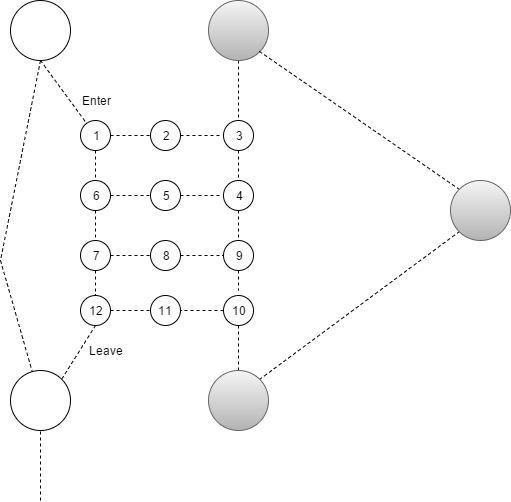
\includegraphics[scale=0.5]{HAMConsistency}\\
\textbf{Figure 5:} Zooming in on the consistency gadget between the choice gadget and the triangle.\\\\
\textbf{Example:}\\
Given a 3SAT formula  $f = (x_1 \lor x_2 \lor x_3) \land (\lnot x_1 \lor \lnot x_2 \lor x_3) \land (\lnot x_1 \lor \lnot x_2 \lor x_3)$\\
We can construct a graph similar to the one in figure 6. For the satisfying assignment $x_1 = 1, x_2 = 0, x_3 = 0$, we can obtain a hamiltonian path by starting at 1, and follwing the pink line to 2.
\begin{center}
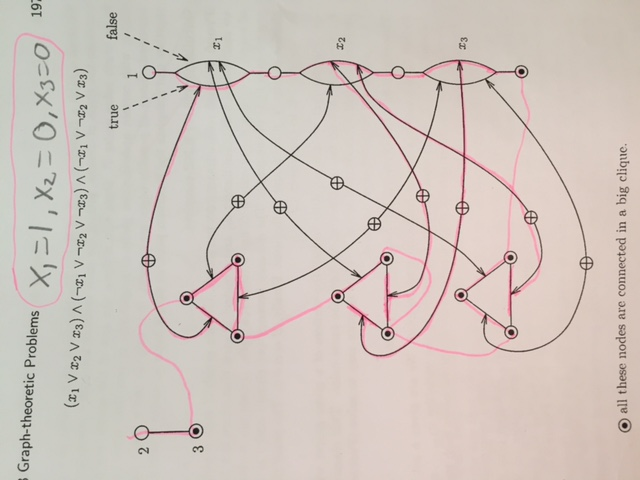
\includegraphics[scale=0.5, angle =-90]{3SATtoHAM}\\
\textbf{Figure 6:} Graph r(f) corresponding to the formula f
\end{center}
\textbf{Polynomial time reduction:}\\
For each variable we make one choice gadget, and for each clause we make one triangle and 3 consistency gadgets.\\\\
$\implies$: \\
Given a satisfying assignment to the input formula f we can show that r(f) has a hamiltonian path: Simply follow the path though the choice gadgets which corresponds to the truth value of the variables. When reaching the clique node after the last choice gadget, we just jump around in the clique and travers the missing edges in each triangle and finally jump to node 3 and then finally 2. 
$\impliedby$: \\
Given that the graph has a hamiltonian path, we show that the input formula is satisfiable: Since there is only two nodes with degree one we can assume the path starts at node 1. Since we know the structure of the graph and the the given hamiltonian path, a truth assignment T is defined by the way the path traverse the choice gadgets and the consistency gadgets along the way. T satisfies the input formula since it makes sure one edge is visited in each triangle. 
\newpage

\section{Cook's theorem and the complexity of variants of SAT.}

\subsection{Beslutningsproblemer og stand-in sprog}
\subsection{P, NP, NPC}
\subsection{Varianter af SAT}
\begin{enumerate}
    \item $SAT \in NPC$
    \item $2SAT \in P$
    \item $3SAT \in NPC$
    \item $NAESAT \in NPC$
    \item $MAX2SAT \in NPC$
\end{enumerate}
\subsection{Cook: $L \in NP \le Circuit SAT$}
\subsection{Circuit SAT $\le$ SAT}
SAT er et slags special case af Circuit SAT hvor det boolske circuit har en helt særlig struktur: En masse AND gates i toppen forbinder alle clauses og resultatet af disse AND gates går til en enkelt OUTPUT gate. Hver clause er OR af dens literals. Og hver literal er en ukendt INPUT gate eller negeringen af en.\\\\
Givet en boolean circuit C konstruerer vi en CNF formula r(C) som følger:\\
Vi ser på hver gate g og dens inputgates $h_1$ og $h_2$. Afhængig af gate typen laver vi følgende forskellige formler:
\begin{enumerate}
	\item AND: Følgende clauses som er logisk ækvivalente med $g \iff (h_1 \land h_2)$
	\begin{center}
		$(\lnot g \lor h_1)(\lnot g \lor h_2)(g \lor \lnot h_1 \lor \lnot h_2)$
	\end{center}
	 Første og anden clause tvinger g til at være 0 hvis $h_1$ eller $h_2$ er 0. Den sidste tvinger g til at være 1 hvis både $h_1$ og $h_2$ er 1.
	\item OR: Følgende clauses som er logisk ækvivalente med $g \iff (h_1 \lor h_2)$
	\begin{center}
		$(g \lor \lnot h_1)(g \lor \lnot h_2)(\lnot g \lor  h_1 \lor h_2)$
	\end{center}
	Første og anden clause tvinger g til at være 1 hvis $h_1$ eller $h_2$ er 1. Sidste clause tvinger g til at være 0 hvis $h_1$ og $h_2$ er 0.
	\item NOT: Følgende clauses som er logisk ævkivalente med $g \iff \lnot h$
	\begin{center}
		$(g \lor h)(\lnot g \lor \lnot h)$
	\end{center}
	Første clause sikrer at g er 1 hvis h er 0, og anden clause sikrer at g er 0 hvis h er 1.
	\item COPY: Følgende clauses som er logisk ækvivalente med $g \iff h$
	\begin{center}
		$(g \lor  \lnot h)(\lnot g \lor h)$
	\end{center}
	Første clause tvinger g til at være 1 hvis h er 1. Anden clause tvinger g til at være 0 hvis h er 0.
	\item CONSTANT: For constant gates tilføjes blot clause $(g)$ eller $(\lnot g)$ afhængig af om gaten er 1 eller 0 hhv. 
	\item OUTPUT: For output gaten tilføjes clause $(g)$. Dermed kan formlen kun være true hvis denne variable og dermed output gaten er true.
\end{enumerate}
Poly tids reduktion da vi max laver 3 clauses for hver gate.\\\\
$\implies$: \\
Givet et tilfredsstillende input til vores Circuit C, hvis vi evaluerer C på dette input, så kan vi sætte boolean variable $g_j = G_j$ hvor $G_j$ er output af den j'te gate af C. Denne tildeling tilfredsstiller vores konstruerede formel.\\\\
$\impliedby$: \\
Givet en tilfredsstillende assignment til formlen F, giv input til Circuit C, den del af F som svarer til input gates i C. Det kan vises med induktion at output for gat j i C er lig med $g_j$ og dermed evaluerer C også til 1.
\subsection{Circuit SAT $\le$ NAESAT}
Genbrug den forrige reduktion og "fyld op" med ny literal z i clauses med 1 og 2 literals. Denne reduktion opfylder nu at $C \in CircuitSAT \iff r(C) \in NAESAT$. De clauses med 3 literals vi har genereret opfylder allerede NAESAT predikatet, og i de andre clauses bruger vi z til at opfylde vores NAESAT constraint. \\\\
Tydeligvis i poly-tids reduktion.\\\
$\implies$: \\
Givet at C kan tilfredsstilles, så kan vi vise at r(C) også kan tilfredsstilles.
Argumentet er delvist det samme som i forrige reduktion: \textit{"Givet et tilfredsstillende input til vores Circuit C, hvis vi evaluerer C på dette input, så kan vi sætte boolean variable $g_j = G_j$ hvor $G_j$ er output af den j'te gate af C."}
Dvs alle clauses har automatisk mindst én sand literal. Og i denne reduktion bruger vi variablen z = false til at sørge for at clauses med 1 og 2 literals også har mindst én  falsk literale.\\\\
$\impliedby$: \\
Hvis der er en tildeling af sandhedsværdier som tilfredsstiller r(C) (i NAESAT forstand), så er det tydeligt at den complementære tildeling også tilfredsstiller i NAESAT forstand. En af disse tildelinger - den hvor z = false - tilfredsstiller også den originale r(C) (den uden z variablen), og dermed også det originale circuit C. \\\\

\subsection{SAT $\le$ 3SAT}
Givet en CNF formel som har clauses med mere eller mindre end 3 literals skal være gøre følgende for hver clause:\\
\begin{enumerate}
    \item Hvis en clause har 1 eller 2 literals, så kopierer vi bare en literal 2 eller 1 gang hhv. Eksempelvis $(x\lor y)$ bliver til $(x \lor y \lor y)$ dette ændrer ikke i semantikken af clausen.
    \item Hvis en clause har mere end 3 literals gør følgende: $ F = (l_1 \lor l_2 \lor A)...$ hvor A er en OR af 2 eller flere literals. Vi indfører nu variabel y og laver nu $F' = (l_1 \lor l_2 \lor y) (\lnot y \lor A)$. Sådan fortsætter vi til A består af en OR af kun  2 literals, da vi så er færdige.
\end{enumerate}
Kører i polytid da vi for hver iteration mindsker en clause med 1 literal indtil vi er færdige. \\\\
$\implies$: Givet en satisfying assignment for F skal vi vise at F' også er satisfied. Vi ser på hvilke dele af F som gøre den satisfied, hvis det er $l_1$ eller $l_2$ så sætter vi y = 0 i $F'$. Hvis $l_1$ og $l_2$ ikke er variablerne som tilfredsstiller f, så må det være en af literals i A, så sætter vi y = 1.\\\\
$\impliedby$: Givet at F' er tilfredsstillet så er F selvfølgelig også uanset sandhedsværdien af y.
\subsection{2SAT $\in$ P}
2SAT algoritme:\\
Konstruer implikationsgraf ud fra en given 2SAT formel: Lav 2n noder, en node for hver variabel og dens negering. Tilføj derefter 2 kanter, $(\lnot a, b)$ og $(\lnot b,a)$ for hver clause $(a \lor b)$. Find stærke sammenhængskomponenter i grafen (cykler) i lineær tid. Tjek vha bfs/dfs for hver variabel om der er en cykel hvor både $x$ og $\lnot x$ indgår. Hvis sådan en variabel eksisterer, så er 2sat formlen unsatisfiable. I alt kan dette gøres i polynomiel tid.
\begin{center}
    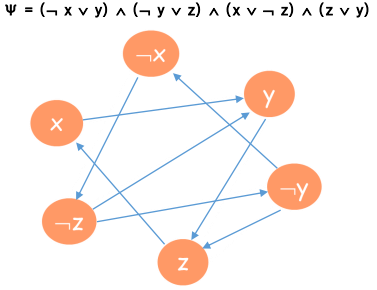
\includegraphics[scale=0.7]{2sat2}
\end{center}
\subsection{3SAT $\le$ MAX2SAT}
Givet en 3SAT formel konstruerer vi en MAX2SAT formel som følger: 
\\
For hver clause $C_i = (\alpha \lor \beta \lor \gamma)$, tilføj følgende 10 clauses:
\begin{center}
    $(\alpha)(\beta)(\gamma)(c_i)\\
    (\lnot \alpha \lor \lnot \beta)(\lnot \beta \lor \lnot \gamma)(\lnot \alpha \lor \lnot \gamma)\\
    (\alpha \lor \lnot c_i)(\beta \lor \lnot c_i)(\gamma \lor \lnot c_i)$
\end{center}
Så hvis 3SAT formlen har m clauses, så har r(x) 10m clauses. The MAX2SAT goal K is equal to 7m.\\\\
Enhver tilfredsstillende assignment for $C_i$ vil tilfredsstille præcis 7 af de tilsvarende 2sat clauses i r(x). Hvis alle literals i 3SAT clausen evaluerer til true, så er hele den første og sidste række tilfredsstillet hvis vi sætter $c_i$ til true. Hvis 2 ud af 3 literals i 3SAT formlen er true, så er 2 clauses tilfredsstillet i hver række, og vi får den 7. uanset sandhedsværdien af $c_i$. Hvis kun en literal er tilfredsstillet er hele 2. række og 1 clause fra første og sidste række tilfredsstillet. Ved at sætte $c_i$ til false opnås 7 clauses.\\
Hvis alle literals evaluerer til false kan max 6 clauses i vores konstruktion tilfredsstilles, hvilket er som ønsket. 
\newpage
\section{NP-complete graph problems.}
\subsection{Beslutningsproblemer og stand-in sprog}
\subsection{P, NP, NPC}
\subsection{Reduktioner}
\subsection{3SAT $\le$ HAMILTONIAN PATH}
\textbf{Theorem 9.7:} HAMILTONIAN PATH is NP-Complete\\\\
We prove this by reducing from 3SAT, which we know is NP-complete.\\\\
We construct a graph G such that G has a Hamiltonian path if and only if the input 3sat formula has a satisfying assignment.\\\\
For each variable we add a choice gadget and join them. For each clause we add a triangle where each edge corresponds to a literal in the clause. For each edge in the triangle, we add a consistency gadget from the edge, to the edge in the corresponding choice gadget. All nodes in all triangles belong to a clique together with the edge following the last choice gadget, and some other node which is the only one adjacent to the last edge in our path (see figure 6.)\\\\
The important thing is that all triangle have at least one edge visited (or actually the 4 nodes on the edges) by the time we get to the clique member after the last choice gadget. If this is not the case then we cannot visit all nodes in a triangle without visiting one of the clique members twice. Recall that edges in the triangles represent literals in the clause - the edges we visit via the choice gadgets are the one for which the corresponding literal make the clause true, and so if no edge is visited, then the clause is false. This is consistent with the fact that we cannot make a hamiltonian cycle. \\\\
Figure 5 show exactly what happens with the consistency gadget. Our path goes through nodes 1,2,3,4... and leaves at 12. It is clear that none of the black nodes are visited. \\\\
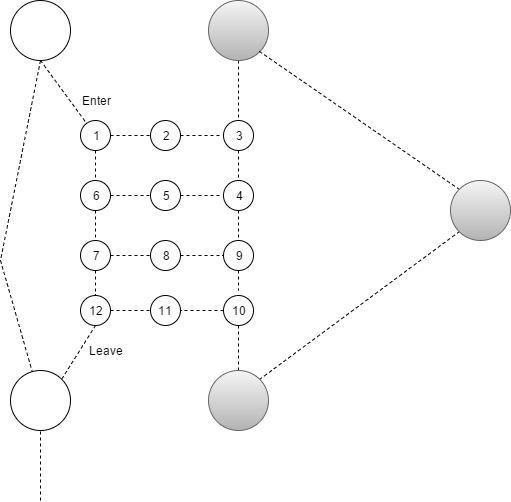
\includegraphics[scale=0.5]{HAMConsistency}\\
\textbf{Figure 5:} Zooming in on the consistency gadget between the choice gadget and the triangle.\\\\
\textbf{Example:}\\
Given a 3SAT formula  $f = (x_1 \lor x_2 \lor x_3) \land (\lnot x_1 \lor \lnot x_2 \lor x_3) \land (\lnot x_1 \lor \lnot x_2 \lor x_3)$\\
We can construct a graph similar to the one in figure 6. For the satisfying assignment $x_1 = 1, x_2 = 0, x_3 = 0$, we can obtain a hamiltonian path by starting at 1, and follwing the pink line to 2.
\begin{center}
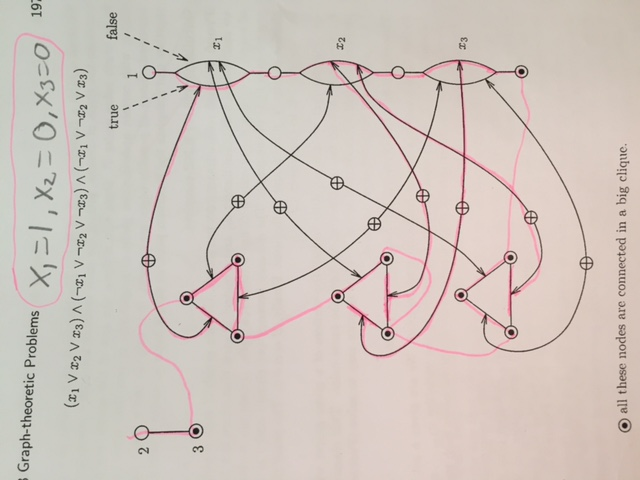
\includegraphics[scale=0.5, angle =-90]{3SATtoHAM}\\
\textbf{Figure 6:} Graph r(f) corresponding to the formula f
\end{center}
\textbf{Polynomial time reduction:}\\
For each variable we make one choice gadget, and for each clause we make one triangle and 3 consistency gadgets.\\\\
$\implies$: \\
Given a satisfying assignment to the input formula f we can show that r(f) has a hamiltonian path: Simply follow the path though the choice gadgets which corresponds to the truth value of the variables. When reaching the clique node after the last choice gadget, we just jump around in the clique and travers the missing edges in each triangle and finally jump to node 3 and then finally 2. 
$\impliedby$: \\
Given that the graph has a hamiltonian path, we show that the input formula is satisfiable: Since there is only two nodes with degree one we can assume the path starts at node 1. Since we know the structure of the graph and the the given hamiltonian path, a truth assignment T is defined by the way the path traverse the choice gadgets and the consistency gadgets along the way. T satisfies the input formula since it makes sure one edge is visited in each triangle. 
\newpage
\subsection{HAMILTONIAN PATH $\le$ TSP}
(with triangle inequality)\\
Given a graph G = (V,E) with n nodes, we make a distance matrix $d_{ij}$ and a budget B such that there is a TSP tour of at most B iff G has a hamiltonian path.\\\\
We enter the distances into the matrix as described below, and set the budget B = n + 1
\begin{gather*}  
d_{ij}: 
\begin{cases}
  d_{ij} = 1 & \text{if (i,j)} \in E\\    
  d_{ij} = 2 & \text{else}
\end{cases}
\end{gather*}
Polynomial time reduction since we just fill a n X n matrix, for each entry looking in E if there is a matching edge.\\\\
$\implies$: \\
Given a hamiltonian path in G we must show that r(G) has a TSP cycle of length at most n + 1. Just follow the hamiltonian path which has length n - 1, now follow an edge back to start, if it is in G then the total length is n, else it becomes n + 1 .  \\\\
$\impliedby$: \\
If we have TSP tour of length at most n + 1 it must use at least n - 1 edges of G, and this will be our hamiltonian path. 
\subsection{3SAT $\le$ INDEPENDENT SET}
\textbf{Theorem 9.4:} INDEPENDENT SET is NP-Complete\\\\
We prove this by reducing from 3SAT, which we know is NP-Complete.\\\\
For this reduction we need a gadget, the triangle. The logic behind this is that, if a graph contains a triangle, then at most one of the nodes can be in the independent set. We restrict the class of graphs we consider, to graphs whose nodes can be partitioned in m disjoint triangles. This ensures that an independent set can contain at most m nodes. \\

For each of the m clauses in our input CNF formula, we create a triangle where the nodes are labeled with the literals of the clause. Next, we add an edge between two nodes in different triangles if and only if the nodes correspond to opposite literals. Adding these edges between opposite literals, ensures that we cannot pick both (as it would not be an independent set). The reduction is completed by setting the independent set goal K = m. \\\\\\
\textbf{Example:}\\
Given a 3CNF formula:  $f =  (x_1 \lor x_2 \lor x_3) \land (\lnot x_1 \lor \lnot x_2 \lor \lnot x_3) \land (\lnot x_1 \lor x_2 \lor x_3)$\\
We construct the graph shown in figure 1. \\\\
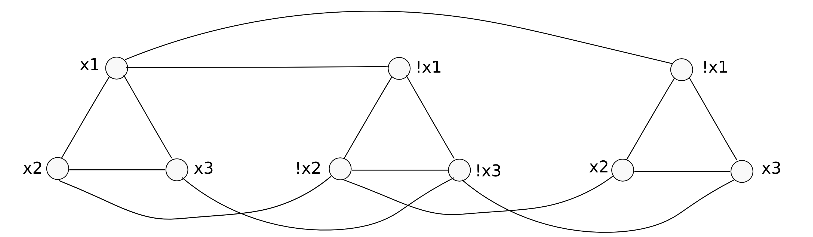
\includegraphics[scale=0.5]{independentset}
\textbf{Figure 1:} Graph r(f) corresponding to the formula f\\\\\\
\textbf{Analysis}\\
For each clause, we just create a triangle. Then we scan every pair of edges and add an edge if the labels are opposite - so the reduction is clearly polynomial.
\\\\
$\implies$ :\\ Given a satisfying assignment for the CNF formula f from above, we must show that the graph, r(f), has an indenpendent set of size K=m. The assignment: $x_1 = 0, x_2 = 1, x_3 = 0$ satisfies the formula, and for our independent set of size K, we pick a node in each triangle which make the corresponding clause true. For the truth assignment we chose above, this means $x_2$ from triangle 1, $\lnot x_1$ in triangle 2, $\lnot x_1$ in triangle 3. (Note that this is not the only valid set since some clauses are satisfied by more than one literals).
\\\\
$\impliedby$ :\\ Given an independent set of size K of r(f), we need to show that there is a satisfying assignment for f. Since it is of size K, it must have one vertex from each triangle, and it cannot contain a variable and its negation. Now, for each vertex in the independent set, we look at the label and assign a truth value to the corresponding variable, so the literal of the label become true. If a variable is not restricted to a truth value by any vertex label, we just assign it some value, since all clauses are already satisfied by the assignments to the other variables.\\\\\\
\textit{Read more in papadimitriou page 188-190.}
\newpage
\subsection{INDEPENDENT SET $\le$ CLIQUE}
The independent set problem asks for a maximum set of vertices of size K. So does the CLIQUE problem. While the independent set problem asks for a set S of vertices where there is no edge between any pair $u,v \in S$, the clique problem ask for the "opposite": a set S where any pair $u,v \in S$ DOES have an edge between them. So the reduction is trivial - we obtain a clique of size K when taking the complementary graph of an independent set of size K.\\\\
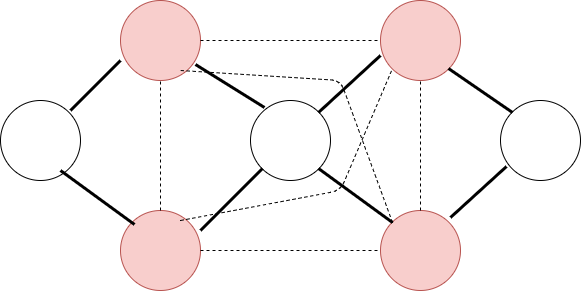
\includegraphics[scale=0.5]{IStoCLIQ}\\
\textbf{Figure 2:} The red nodes are the maximum independent set I - the dotted lines completes the complementary graph of I. A clique of same size.
\\\\\\
\textit{Read more in papadimitriou page 190.}
\newpage
\subsection{INDEPENDENT SET $\le$ VERTEX COVER}
While independent set is a maximization problem, vertex cover is a minimization problem. For a graph G = (V,E) and a max independent set $I \subseteq V$, the minimum vertex cover set is just $V-I$.\\\\
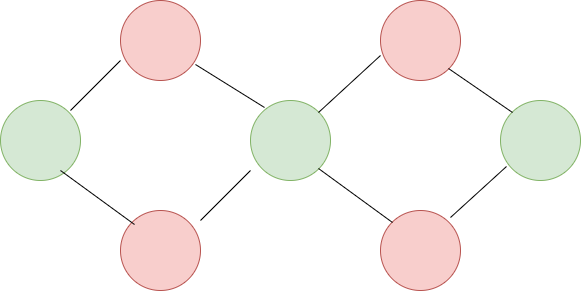
\includegraphics[scale=0.5]{IStoCOVER}\\
\textbf{Figure 3:} The red node forms the maximum independent set. The green form the minimal vertex cover.
\\\\\\
\textit{Read more in papadimitriou page 190.}
\newpage


\newpage

\section{NP-complete problems involving sets and numbers.}
\subsection{Beslutningsproblemer og stand-in sprog}
\subsection{P, NP, NPC}
\subsection{Reduktioner}
\subsection{3SAT $\le$ TRIPARTITE MATCHING}
For this reduction we use a combined choice- and consistency gadget. We create one for each variable $x_i$. Each one of such gadget will have k boys, k girls and 2k homes. Where k is equal to the highest occurrence of $x_i$ or $\lnot x_i$.
The uneven numbered homes represent occurrences of x, and the other of $\lnot x$. The boys and girls of these gadgets are only paired with the homes of the same gadget. If a matching exists then $b_i$ is matched with either $g_i$ and $h_{2i}$, or to $g_{i-1}$ and $h_{2i-1}$. The first matching is taken to mean that x = 1 and the second that x = 0.
\\\\
For each clause we add another pair of boy and girl. These will be paired with the corresponding literals in the gadgets. The idea is that if one of these three homes was left unoccupied when the variables were assigned truth values, this means that it corresponds to a true literal, and therefore the clause is satisfied. \textbf{If all three literals in c are false, then the corresponding b/g pair cannot be matched with a home.} \\\\
There are always L extra homes in this construction, and to make sure they can be matched, we introduce L more boy/girl pairs. These pairs all paired with every home in the construction. So these L boy/girl pairs are "easy to please" and are just used to pair the leftover homes. \\\\

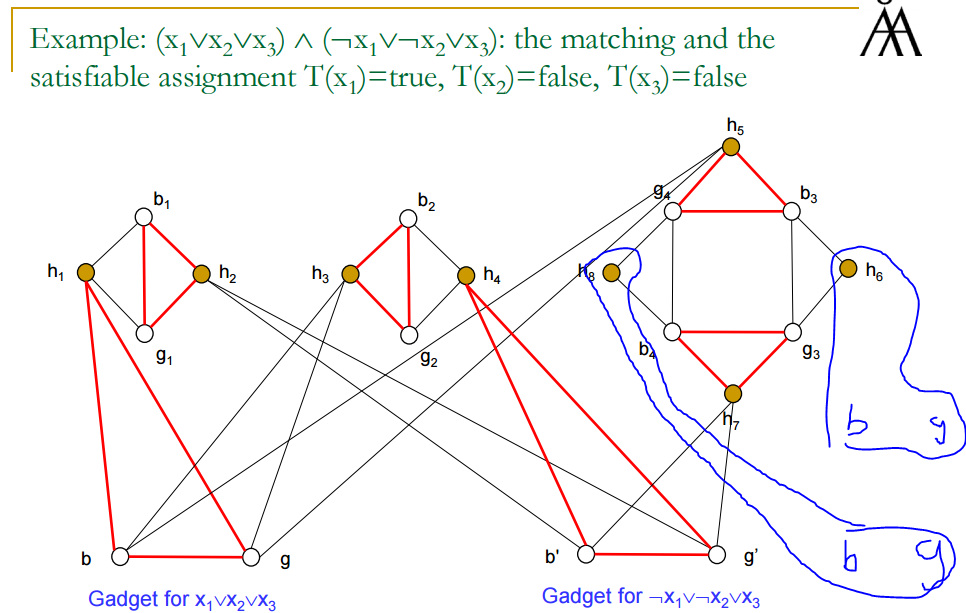
\includegraphics[scale=0.5]{tripartite}
\\
\textbf{Polynomial:} For each variable we make a gadget with at most m boys/girls and 2m homes. For each clause we make a b/g pair. And for each extra home another b/g pair. So it is polynomial.
\\\\
$\implies:$ \\ TODO
\\\\ 
$\impliedby:$ \\ TODO

\newpage
\subsection{Corollary: EXACT COVER BY 3-SETS, SET COVERING AND SET PACKING ARE NP COMPLETE}
TRIPARTITE MATCHING is a special case of EXACT COVER BY 3-SETS. And EXACT COVER BY 3-SETS is a special case of both SET COVER and SET PACKING.\\\\ (https://people.eecs.berkeley.edu/~vazirani/algorithms/chap8.pdf)
\subsubsection{TRIPARTITE MATCHING $\le$ EXACT COVER BY 3-SETS}
Given a TRIPARTITE MATCHING instance: let the EXCB3-S subsets be the same as in the TRIPARTITE MATCHING instance. The EXCB3-S universe is obtained by the union of B G and H.\\\\
Think of EXCB3-S as kind of the same problem but where you can match 3 Boys, or 2 girls and 1 home etc. 
\subsubsection{EXACT COVER BY 3-SETS $\le$ SET COVERING}
EXACT COVER BY 3-SETS instances are a subset of all SET COVERING instances, so the is easy. Nothing is changed and the Budget B = m from the EXCB3-S instance.

\subsubsection{NODE COVER $\le$ 
SET COVERING}
SET COVER is a generalization of NODE COVER. In our construction the universe is all edges in the NODE COVER instance. The subsets are obtained as follows: For each node in the graph, all adjacent edges form a subset.
\subsubsection{EXACT COVER BY 3-SETS $\le$
SET PACKING}
Set the SET PACKING goal k to be m. Then there is a 3-SET cover of size m iff there is a SET PACKING of size m. (Since the input set is 3m). Rest is unchanged.  
\newpage
\subsection{EXACT COVER BY 3-SETS $\le$ KNAPSACK}
Once again we will prove a problem NP hard by showing that a special case is NP hard. The special case of KNAPSACK where $v_i = w_i$ and goal $K = W$ is called SUBSET SUM. (see definition in first section).\\\\
In our construction we think of the 3-sets as binary vectors in $\{0,1\}^{3m}$. And the i'th bit will be 1 iff the i'th element is contained with this particular 3-set. Therefore in each vector, only 3 ones will appear. The vectors can be thought of as binary integers, and set union now resembles integer addition and the goal is to find vectors which sum up to the all 1's vector. \\\\
But binary addition has a carry, which could break the bi-implication. For example 0011 + 0101 + 0111 = 1111, but the sets $\{3,4\}$,$\{2,4\}$,$\{2,3,4\}$ are not disjoint, and their union is not $\{1,2,3,4\}$.\\
To fix this, we think of the numbers in base n+1 instead of 2. since we have n vectors, there can never be a carry.\\\\
The weight goal of $2^{3m}-1$ completes the reduction.\\\\
$\implies$ :\\ If there is an exact cover by 3-sets, then the bit vectors in our construction corresponding to the exact cover will provide a number equal to the wanted K.\\\\
$\impliedby$ :\\ Since we can include every number once, and there is no carry, then there must be vectors which add up to K, and therefore also an exact cover by 3-sets.
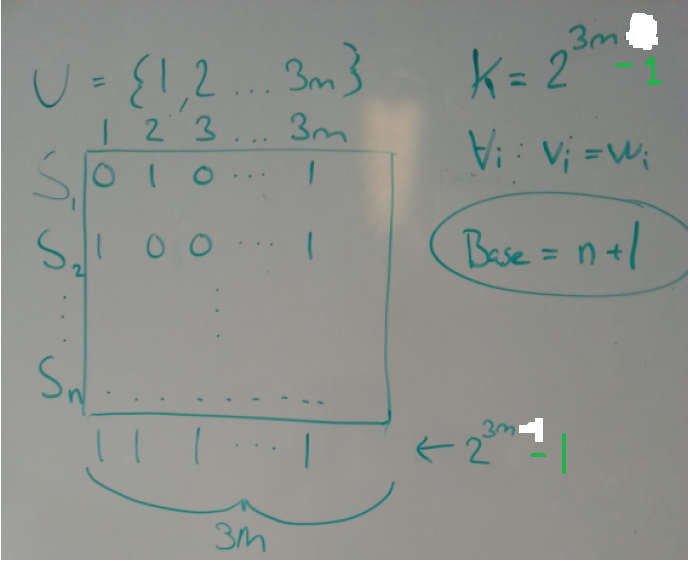
\includegraphics[scale=0.5]{knapsack}
\newpage




\newpage

\section{Approximation algorithms.}
\subsection{Disposition}
\begin{enumerate}
    \item P, NP, NPC
    \item Løsning af NPC problemer
    \item Approximations algoritmer
    \item Approx schemes
    \item Algo design 
    \item vertex cover
    \item TSP
\end{enumerate}
\newpage
\subsection{P, NP, NPC}
\subsection{Løsninger af NPC problemer}
NPC indeholder mange problemer som vi gerne vil løse på en eller anden måde. Vi har følgende muligheder:
\begin{itemize}
	\item Små instanser kan ofte løses selvom udførselstiden er exponentiel
	\item Der kan være nogle special cases instanser som kan løses i polynomiel tid		\item Heuristics
	\item Approximations algoritmer	
\end{itemize}
\subsection{Approx. algoritmer}
En approximerings algoritme returnerer en valid løsning men som ikke er optimal. Den kører i polynomiel tid.\\

En algoritme for et givent problem har en approximations ratio p(n) hvis, for alle inputs af størrelse n,  den returnerede løsning med cost C er indenfor en faktor p(n) af den optimale løsning med cost $C^*$:
\begin{center}
$max(\frac{C}{C^*},\frac{C^*}{C})\le p(n)$
\end{center}
\subsection{Approx. schemes}
\subsection{Design}

\subsection{Vertex cover}
Følgende algoritme er en 2-Approximations algoritme. 
\begin{center}
	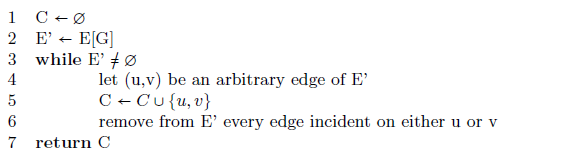
\includegraphics[scale=0.7]{ApproxVertexCover}
\end{center}
Bevis:\\
Først og fremmest så returnerer algoritmen en valid node cover: for hver iteration vælges en tilfældig kant, og alle kanter som ligger op af de to noder bliver fjernet. Dette sker indtil der ikke er flere kanter, og dermed er alle kanter dækket.\\\\
Lad A være de tilfældigt udvalgte kanter som vælges i linje 4. For alle noder i A må mindst én af endpoint noderne være i $C^*$, dermed har vi en lower bound på den optimale løsning:
\begin{center}
	$|C^*| \ge |A|$
\end{center}
Hver gang vi udvælger en kant i linje 4, så inkluderer vi 2 noder i vores vertex cover. Dermed har vi:
\begin{center}
	$|C| = 2|A|$
\end{center}
Ved at kombinere disse kan vi udlede at denne algoritme er en 2-approximations algoritme:
\begin{center}
 	$|C| = 2|A|$
 	\\ \qquad  $\le 2|C^*|$
\end{center}
Ovenstående siger os at cost af den producerede løsning maximalt kan være 2 gange cost af optimal løsning.
\subsection{Metric TSP}
Følgende er en beskrivelse af en 2-approximations algoritme til TSP som overholder trekantsuligheden.\\ (Dvs cost funktionen $c(A) = \sum\limits_{(u,v)\in A } c(u,v)$\\ tilfredstiller at for alle noder $u,v,w \in V: c(u,w) \le c(u,v) + c(v,w)$ )\\
\begin{center}
	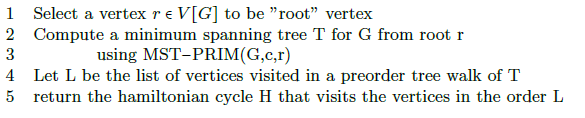
\includegraphics[scale=0.7]{tspApprox}
\end{center}

Algoritmen genererer et minimum spanning tree vha prims algoritme $(O(|V^2|))$, og returnerer en hamiltonian path bestående af  en noderne besøgt i en depth first preorder traversal af dette træ.\\ 

\begin{center}
	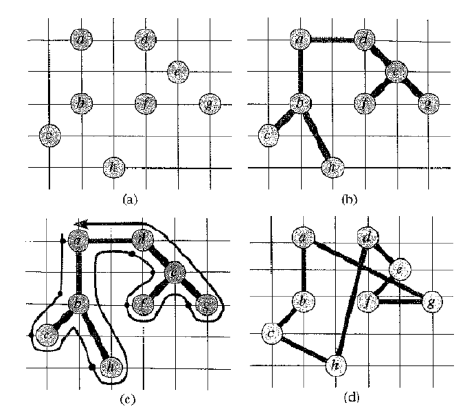
\includegraphics[scale=0.5]{ApproxMetricTSP}\\ Eksempel\\
	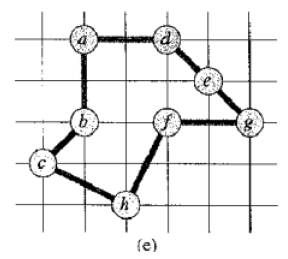
\includegraphics[scale=0.5]{tspMetricOptimal}\\ Optimal 
\end{center}
\textbf{2-approximation:} Lad $H^*$ være en optimal tour. Hvis vi fjerner en kant fra en tour, så får vi et spanning tree. Derfor kan vi bruge vægten af et MST T som lower bound:
\begin{center}
 $c(T) \le c(H^*)$
\end{center}
Et full preorder walk FW lister knuderne hver gang de besøges. Det er let at se at hver kant i træet traverseres præcis 2 gange. Dermed har vi:
\begin{center}
	$c(FW) = 2c(T)$
\end{center}
Og ved at kombinere disse to får vi:
\begin{center}
	$c(FW) \le 2c(H^*)$ 
\end{center}
Altså at costen af vores full walk er indenfor en faktor af  2 af costen af en optimal tour. Men FW er ikke en tour da den besøger nogle noder mere end 1 gang. Dog kan vi bruge vores antagelse omkring trekantsuligheden, og slette noder i vores full walk uden at øge costen. Derfor sletter vi alle "anden forekomster" af noder i vores full walk, og den resterende liste udgør en tour. For eksemplet ovenfor reduceres listen:
\begin{center}
	a,b,c,b,h,b,a,d,e,f,e,g,e,d,a $\rightarrow$ a,b,c,h,d,e,f,g
\end{center}
Den reducerede liste udgør nu vores approximative tour H som returneres af algoritmen. Da H er opnået ved at slette noder fra full walk FW ved vi at costen af H er mindre eller lig med costen af FW:
\begin{center}
	$c(H) \le c(FW)$
\end{center}
Og ved at kombinere dette og det forrige udtryk kan vi konkludere at:
\begin{center}
	$c(H) \le 2c(H^*)$
\end{center}
\section{Problemer og flere reduktioner}
\subsection{INDEPENDENT SET}
\textbf{Given:} Graph G = (V,E), target K. \\
\textbf{Question:} Does there exist $I \subseteq V$ such that $|I| \geq K$\\ and for all $u,v\in I$ we have $(u,v) \notin E$? 
\subsection{CLIQUE}
\textbf{Given:} Graph G = (V,E), target K. \\
\textbf{Question:} Does there exist $C \subseteq V$ such that $|C| \geq K$\\ and for all $u,v\in C$ we have $(u,v) \in E$?
\subsection{VERTEX COVER}
\textbf{Given:} Graph G = (V,E), budget B. \\
\textbf{Question:} Does there exist $C \subseteq V$ such that $|C| \leq B$\\
and for all $(u,v) \in E$ we have $(u \in C \lor v \in C)$?
\subsection{MAX CUT}
\textbf{Given:} Graph G = (V,E), target K. \\
\textbf{Question:} Does there exist a cut  $(S,V\setminus S)$ of size at least K?\\
\subsection{MAX BISECTION}
\textbf{Given:} Graph G = (V,E), target K.\\
\textbf{Question:} Does there exist a cut  $(S,V\setminus S)$ of size at least K, such that $|S| =  |V \setminus S|$?
\subsection{BISECTION WIDTH}
\textbf{Given:} Graph G = (V,E), target K.\\
\textbf{Question:} Does there exist a cut  $(S,V\setminus S)$ of size at most K, such that $|S| =  |V \setminus S|$?
\subsection{HAMILTONIAN PATH}
\textbf{Given:} Graph G = (V,E).\\
\textbf{Question:} Does G have a path that visits every vertex exactly once?\\
\subsection{TSP}
\textbf{Given:} Distance matrix D, target t. \\
\textbf{Question:} Is there a tour of length at most t that visits every node in the graph defined by D exactly once?\\
\subsection{SET COVERING}
\textbf{Given:} 
A set U(universe). A collection of subsets $S_1,S_2,...,S_n \subseteq U$\\
\textbf{Question:} Does there exist B subsets whose union is U?
\subsection{EXACT COVER BY 3-SETS}
\textbf{Given:} 
A set U of size 3m. A collection of subsets $S_1,S_2,...,S_n \subseteq U$ of size three.\\
\textbf{Question:} Does there exist m subsets which cover U exactly? 
\subsection{TRIPARTITE MATCHING}
\textbf{Given:} 
Three sets B, G, H of size n. A collection of triples $T \subseteq B \bigtimes G \bigtimes H.$\\
\textbf{Question:} Does there exist n triples such that every element of B, G and H is contained in exactly one of these triples?
\subsection{SET PACKING}
\textbf{Given:} 
A set U. A collection of subsets $S_1,S_2,...,S_n \subseteq U$. A goal K.\\
\textbf{Question:} Does there exist k pairwise disjoint subsets?
\subsection{KNAPSACK}
\textbf{Given:} 
N items. Item i has value $v_i$ and weight $w_i$, both positive integers. A max weight W. And a goal K. \\
\textbf{Question:} is there a subset of the N items such that the total weight is at most W and that the total value is at least K?
\subsection{SUBSET SUM (SPECIAL CASE OF KNAPSACK)}
In this version of knapsack an items value is equal to its weight, and the goal K is equal to the max weight W. So, we are given a set of N integers and an integer K and ask if there is a subset of the given integers that adds up to K.
\subsection{BIN PACKING}
\textbf{Given:} 
N positive integers and two more integers C(capacity) and B(number of bins).  \\
\textbf{Question:} can these numbers be partitioned into B subsets, each of which has a total sum of at most C?
\subsection{NAESAT $\le$ MAX CUT}
\textbf{Theorem 9.5:} MAX CUT is NP-Complete\\\\
We prove this by reducing from NAESAT, which we know is NP-complete.\\\\
We construct a graph G = (V,E), and a goal K such that there is a way to separate the nodes og G in to two sets S and V-S with K or more edges  going from one set to the other, if and only if there is a truth assignment for our NAESAT formula f which satisfies f. We allow more than one edge between two vertices, and each such edge contributes one to the cut. 
\\\\
Our input formula has m clauses and n variables, and we constuct a graph with 2n nodes - one for each variable and it's negation. For each clause, we add edges to our graph to form triangles. If two literals of a clause are the same, for example $(x \lor y \lor y)$, (which is equivalent to $(x \lor y)$), we just add two edges between the nodes representing the two destinct literals. The point of the triangles and the two edges between same literals, is that for both constructs, the cut is always two. Now we add an edge between variables and their negation, and set our target K = n + 2m. \textbf{The n is for cutting the horizontal edges, and 2m is because we need to cut each triangle (each clause) - if we don't, then it is possible for all literals in a single clause to be true (and then it's not naesat))}. This completes the reduction.\\\\
\textbf{Example:}\\
Given a NAESAT formula:  $f =  (x_1 \lor x_2) \land (x_1 \lor \lnot x_3) \land (\lnot x_1 \lor \lnot x_2 \lor x_3)$\\
We can construct the graph shown in figure 4. The green edges come from the first clause, red the second clause, and blue the third clause.\\
\begin{center}
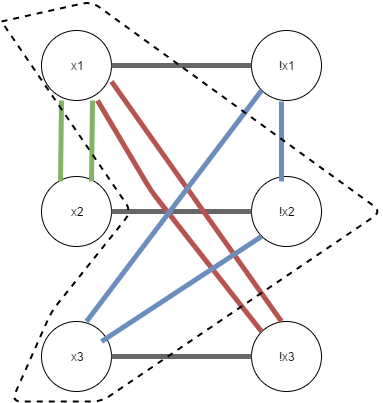
\includegraphics[scale=0.5]{NAESATtoMAXCUT}\\
\textbf{Figure 4:} Graph r(f) corresponding to the formula f
\end{center}
\textbf{Analysis:}\\
For each variable we add two nodes and one edge between them. For each clause we add at most 3 edges. So the reduction is polynomial.\\\\
$\implies$ :\\
Given a satisfying naesat assignment for f, we must show that r(f) has a cut of size at least K. $x_1 = 1, x_2 = 0, x_3 = 1$ is a satisfying assignment for f. We have 3 variables and 3 clauses, so the target K is $2*3+3 = 9$. The cut of 9 is obtained by cutting the vertices within the dotted line in the example above. 
\\\\
$\impliedby$ :\\
Given a cut of size at least K of r(f), we must show that there is a satisfying naesat assignment for x. Here we just take the truth values of the nodes in our cut set.
\\\\\\
\textit{Read more in papadimitriou page 191-192.}
\newpage







\end{document}
